\documentclass[border=10pt]{standalone}

\usepackage{tikz}
\usepackage{tikzsymbols}
\usetikzlibrary{calc,patterns,shapes.geometric}

\def\centerarc[#1](#2)(#3:#4:#5){\draw[#1] ($(#2)+({#5*cos(#3)},{#5*sin(#3)})$) arc (#3:#4:#5);}

\begin{document}
	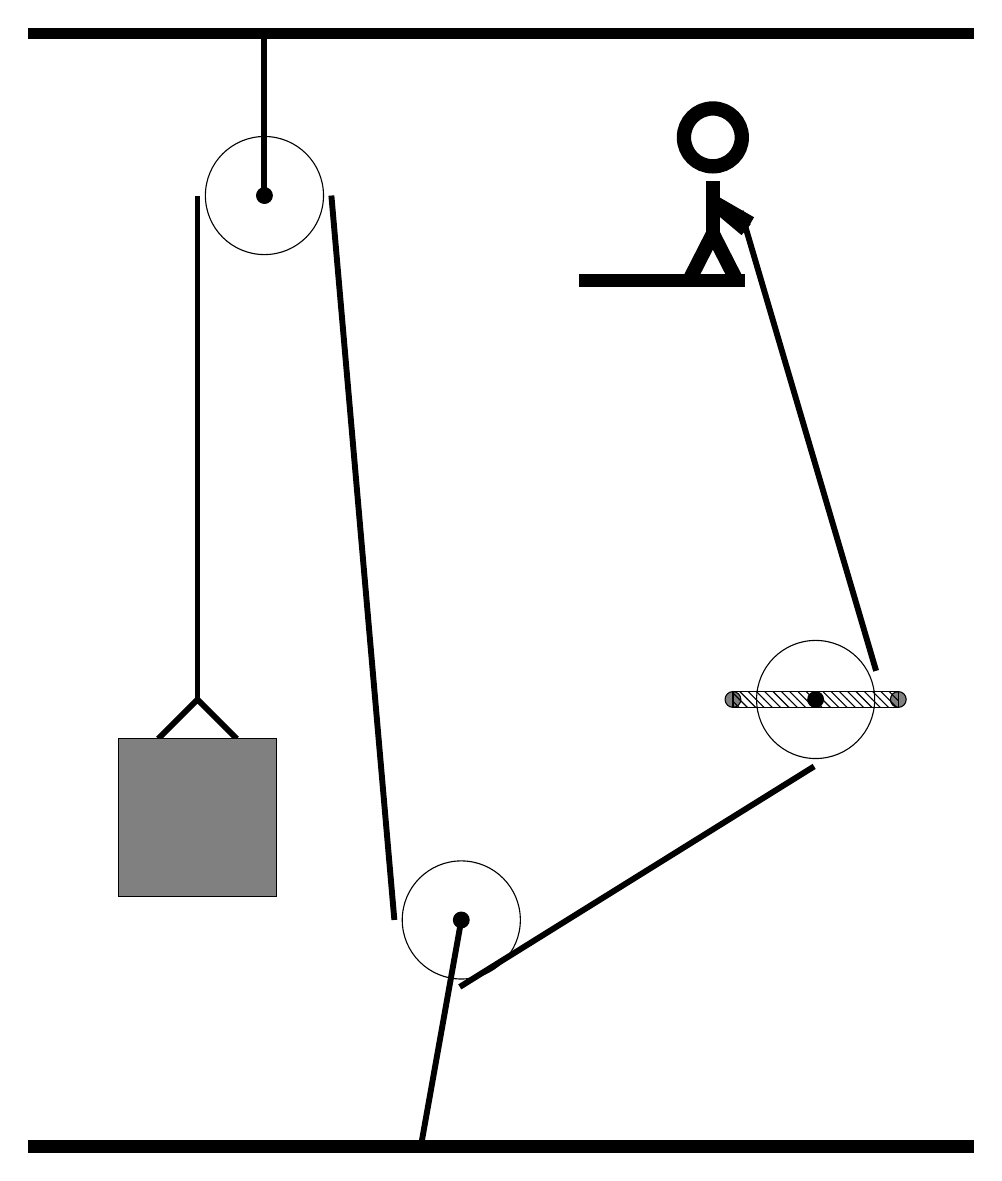
\begin{tikzpicture}
		%%%%% START %%%%%
		\draw[fill=black] (-2, 14) rectangle (10, 14.125);
		
		\draw (1, 12) circle (0.75);
		\draw[fill=black] (1, 12) circle (0.1);
		\draw[line width=0.75mm] (1, 14) -- (1, 12);
		
		\draw (3.5, 2.8) circle (0.75);
		\draw[fill=black] (3.5, 2.8) circle (0.1);
		\draw[line width=0.75mm] (3.5, 2.8) -- (3.0, 0);
		
		\draw[fill=white](8, 5.6) circle (0.75);
		\draw[fill=black] (8, 5.6) circle (0.1);
		\draw[fill=black!50] (9.05, 5.6) circle (0.1);
		\draw[fill=black!50] (6.95, 5.6) circle (0.1);
		\draw[pattern=north west lines, pattern color=black] (6.95, 5.7) rectangle (9.05, 5.5);
		
		\draw[line width=0.75mm](-0.35, 5.1) --  (0.15, 5.6) -- (0.65, 5.1);
		\draw[fill=black!50] (-0.85, 5.1) rectangle (1.15, 3.1);
		
		\draw[line width=0.75mm](0.15, 12) -- (0.15, 5.6);
		\centerarc[line width=0.75mm](1, 12)(180:0:0.85)
		\draw[line width=0.75mm](1.85, 12) -- (2.65, 2.8);
		\centerarc[line width=0.75mm](3.5, 2.8)(180:300:0.85);
		\draw[line width=0.75mm](3.481, 1.95) -- (7.981, 4.75);
		\centerarc[line width=0.75mm](8, 5.6)(300:390:0.85);
		\draw[line width=0.75mm](8.768, 5.964) -- (7.05, 11.8);
		
		\node at (6.75, 12) {\Strichmaxerl[10][-220][-30]};
		\draw[fill=black] (5, 11) rectangle (7.1, 10.85);
		
		\draw[fill=black] (-2, 0) rectangle (10, -0.15);
		%%%%% END %%%%%
	\end{tikzpicture}
\end{document}